\section{Method}

In the consecutive parts we discuss the parameters relevant for the conducted
experiments. This includes decisions we made for the setup as a whole
(dataset, pre processing) but also detail decisions regarding for example
the implementation of a specific model. The source code based on the
Tensorflow framework~\cite{tensorflow15} will be made available through
GitHub.

\subsection{Dataset and preprocessing}

Though there are several \gls{mri} and \gls{ct} datasets available, for
instance \gls{oasis}~\cite{OASIS} or \gls{adni}~\cite{ADNI}, public datasets
in which both modalities are present for the same subject are to date rare. To
our knowledge there are only two public databases available that disclose
\gls{mri} and \gls{ct} volumes for the same subjects, namely the \gls{rire}
project~\cite{RIRE} and the Cancer Imaging Archive~\cite{CIA}. For the present
work we limited ourselves to the imaging data of the \gls{rire} project, as we
found that it involved a simpler preprocessing pipeline.

The \gls{rire} dataset contains multi-modality imaging data of about \num{19}
patients. In \Cref{tab:rire} we present the total number of modalities
available. Beside of the \gls{ct} modalities the dataset also provides
\gls{pet} volumes for some subjects. Beside the common \gls{t1} and \gls{t2}
weightes sequences, there are also \gls{pd} and \gls{mp} \gls{rage} sequences
used to obtain the different \gls{mri} volumes. Furtheremore some modalities
were also available in a rectified version, which we, however, did not use.
\begin{table}[h]
  \centering
  \begin{tabular}{*{6}{c}}
    \toprule
             & \multicolumn{4}{c}{\gls{mri}} & \\
    \cmidrule{2-5}
    \gls{ct} & \gls{pd} & \gls{t1} & \gls{t2} & \gls{mp} \gls{rage} & \gls{pet} \\
    \midrule
    \num{17} & \num{14} & \num{19} & \num{18} & \num{9} & \num{8} \\
             & \num{12} & \num{17} & \num{16} & \num{9} & \num{6} \\
    \bottomrule
  \end{tabular}
  \caption{Subject statistics with respect of the available imaging
    modalities of the \gls{rire} dataset. The second table only accounts for
    subjects with available \gls{ct} data.
  }\label{tab:rire}
\end{table}
For the second row in \Cref{tab:rire} we only account for subjects that have
a \gls{ct} volume to count. For the subsequent steps we decided to select the
\gls{t1} weighted \gls{mri} as it had the highest subject count.

The modality data for each subject can be downloaded from the website of the
\gls{rire} project, see Ref.~\cite{RIRE}. The first preprocessing step,
depicted in \Cref{fig:conversion}, involves the extraction, decompression and
conversion of the downloaded data. After extraction and decompression the
volumetric data presents itself as \gls{mhd}. We convert the \gls{mhd} files
to the self-contained \gls{nifti} format through the Python front-end of the
\gls{itk} library. 
\begin{figure}[h]
  \centering
  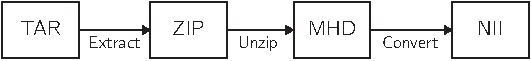
\includegraphics[width=\linewidth]{figure/conversion.pdf}
  \caption{Dataset conversion from \gls{mhd} to \gls{nifti} format.
	}\label{fig:conversion}
\end{figure}
We were able to co-register the modalities using~\cite{SPM12} and the
highest interpolation order. In the same step we also resliced the volumes
to have a homogenous voxel size as the RIRE dataset has only a low resolution
in the sagittal plane.


Finally we used~\cite{Nibabel} to load the aligned volumes and convert them
into Tensorflow's tfrecord format and split them into a validation set of
4 and a training set of 13 patients. Inside the tensorflow input pipeline
we normalized the value range of each volume to $[0,1]$. For two dimensional
models we padded the horizontal slices to $384\times384$. For three
dimensional models we used $260\times340\times360$ (Depth x Height x Width).

\subsection{Network}

As generative adversarial networks we decided to use pix2pix~\cite{Isola16}
as it has already shown great results in the task of color image to image
translation and context-aware 3d synthesis~\cite{Nie16} which uses a simpler
generator but accounts for 3d structures.

As convolutional encoder-decoder network we chose u-net~\cite{Ronneberger15}
as it was able to compete with much larger models in the task of semantic
segmentation~\cite{Badrinarayanan15}. Further our implementation of pix2pix
uses u-net as generator network, hence we are able to evaluate the impact
of the adversarial min-max approach.

Eventually we want to evaluate a new network and training approach novel to
medical computer vision~\cite{Karras17}.

\subsubsection{U-Net}


\subsubsection{Pix2Pix}

\subsubsection{3D Synthesis}

\subsection{Losses}

\subsubsection{Distance Losses}

As norm losses we refer to the mean absolute error ($L1$ loss) and the
mean squared error ($L2$ loss).

\subsubsection{Gradient Losses}

The gradient (difference) loss is used in the framework of context-aware
3d synthesis~\cite{Nie16} in addition to the norm loss.

\subsubsection{Signal Losses}

From signal processing PSNR,SSE

\subsubsection{Adversarial Loss}

Least-squared adversarial loss, standard adversarial loss. BEGAN loss?


\subsection{Augmentation}

\subsubsection{Random Crop}
\subsubsection{Rotation}
\subsubsection{Contast Adjustment}

